% This is samplepaper.tex, a sample chapter demonstrating the
% LLNCS macro package for Springer Computer Science proceedings;
% Version 2.20 of 2017/10/04
%
\documentclass[runningheads]{llncs}
%
\usepackage{graphicx}
\usepackage{amsmath}
\usepackage[boxed,ruled]{algorithm2e}
\usepackage{todonotes}
\usepackage{booktabs}
\usepackage{tabularx}
% Used for displaying a sample figure. If possible, figure files should
% be included in EPS format.
%
% If you use the hyperref package, please uncomment the following line
% to display URLs in blue roman font according to Springer's eBook style:
% \renewcommand\UrlFont{\color{blue}\rmfamily}
\usepackage[numbers,sort&compress]{natbib}
\begin{document}
%
\title{Learning Spectral Representations:\\ Semantic Memory and the\\ Information Dynamics of Thinking}
%
\titlerunning{Learning Spectral Representations}
% If the paper title is too long for the running head, you can set
% an abbreviated paper title here
%
\author{Steve~Homer\inst{1}\orcidID{0000-1111-2222-3333} \and
Geraint~A.~Wiggins\inst{1,2}\orcidID{0000-0002-1587-112X}}
%
\authorrunning{S.~Homer and G.~A.~Wiggins}
% First names are abbreviated in the running head.
% If there are more than two authors, 'et al.' is used.
%
\institute{AI Lab, Vrije Universiteit Brussel, 1050 Brussels, Belgium \and
School of Electronic Engineering and Computer Science,\\Queen Mary University of London, Mile End Road, London E1 4FZ, UK \\
\email{steven.t.homer@gmail.com,geraint@ai.vub.ac.be}}
%
\maketitle              % typeset the header of the contribution
%
\begin{abstract}
The abstract should briefly summarize the contents of the paper in
150--250 words.

\keywords{Statistical learning  \and Representation Learning \and Information Dynamics.}
\end{abstract}
%
%
%
\section{Introduction}
This paper presents progress in statistical knowledge representation applied to auditory input, specifically speech. The work has been conducted in the context of a longer-term project, on the Information Dynamics of Thinking (IDyOT). Until the current publication, the work has focused either on theoretical explication \cite{Wiggins12,WigginsForth15,ForthAgresEtAl16,vanderVeldeForthEtAl17,Wiggins18}, or on statistical modelling applied to textual data \cite{WigginsSanjekdar19}. In this paper, we begin to explore the potential of the IDyOT theory to learn its own representations and build hierarchical ``deep'' representations of meaning. At this stage, we do not claim that these representations are cognitively valid; rather we attempt just to demonstrate that the proposal is capable of learning from data in the way proposed, and that the representations produced are credible as the output of a human-like learning system. The key contribution of the present paper is the use of spectral approaches to knowledge representation and the extraction of knowledge from time-variant speech information in the context of structural analysis by statistical model.

In the following sections, we first outline the context of the Information Dynamics of Thinking project, and summarise it. We then explain the detail of our implementation. We detail the empirical studies we have conducted to test whether the theory identifies perceptual and semantic categories as predicted. Finally, we discuss the prospects for future work on the model.
\section{Background}
\subsection{Overview}
\begin{figure}[t]
    \centering
    \resizebox{.9\linewidth}{!}{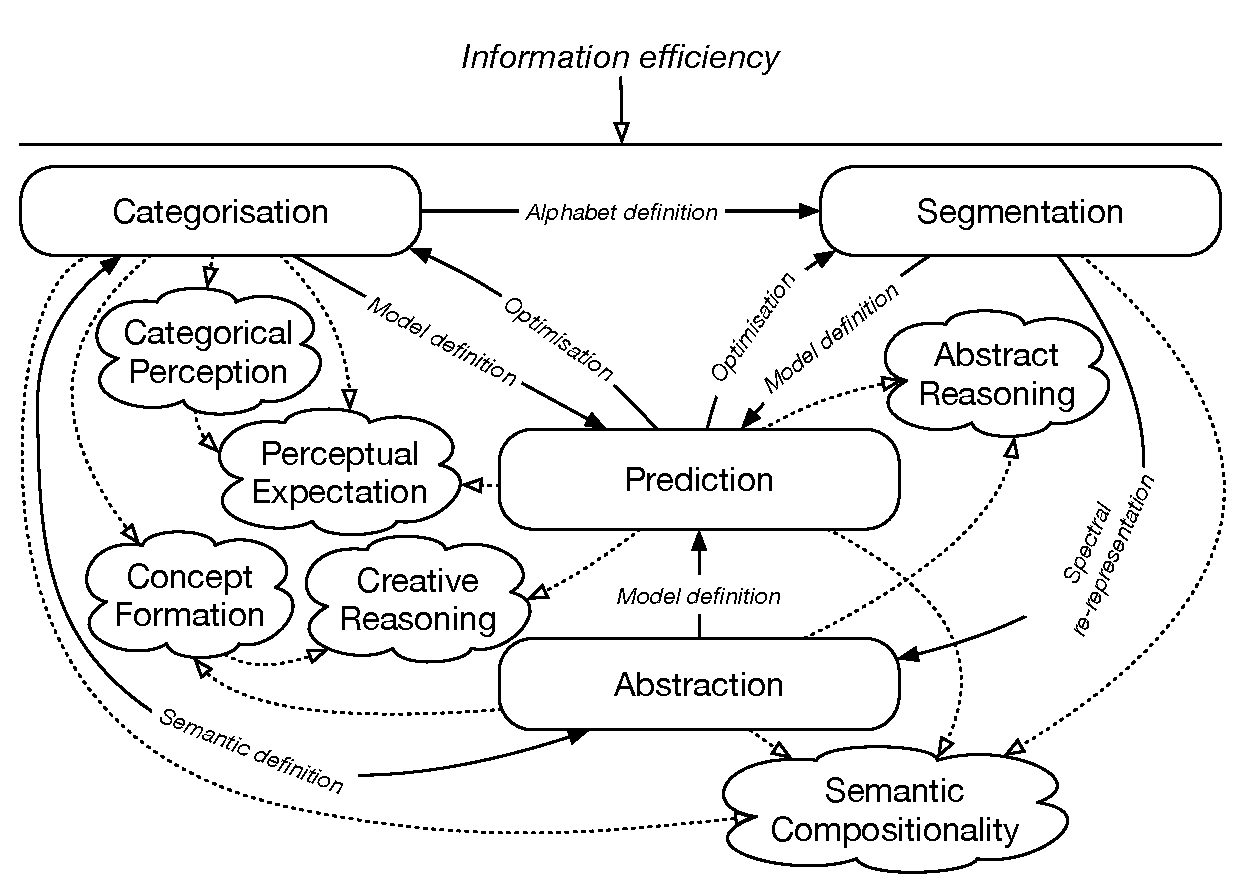
\includegraphics{pix/overview}}
    \caption{Overview of IDyOT components and operation cycle. Rounded boxes are the main IDyOT processes. Cloud shapes represent the phenomena explicated. Arrows are labelled with the operations that connect the main processes. The whole is guided by the information efficiency criterion. Figure and caption reproduced under CC-BY license \cite{WigginsSanjekdar19}.}
    \label{fig:IDyOToverview}
\end{figure}
The theory of Information Dynamics of Thinking (IDyOT) is an attempt to capture in an implemented computational model a hypothetical fundamental cognitive process. That process, it is claimed, drives cognition and action in a mind. The theory draws together the processes of (implicit, non-conscious) learning, segmentation of sequences in time, construction of categorical perceptual and semantic representations, and abstraction of data into ontological hierarchies. The motivation of the theory is to be able to predict what happens next in the world, so it accords mostly with the approach of Clark \cite{Clark13}. Like many such theories, it is based on statistical modelling (viewed as a simulation of cognitive process, not as a model of data) and Shannon information theory \citep{Shannon48}. The theory is formulated as one of ``information dynamics'', and not as one of ``free energy''  \citep{Friston10}, because there is evidence (from music cognition studies  \citep{Huron06,PearceWiggins12,HansenPearce14}) that humans are directly sensitive to the quantity of Shannon entropy in perceived data, and so  grander physical metaphor is superfluous.

The IDyOT process is illustrated in Fig.~\ref{fig:IDyOToverview}. It operates over 
% this bit taken directly from Frontiers paper - needs reworking
input sequences at a given basic level of representation---here, the vectors of a Fourier Transform of human speech. These sequences are segmented using boundary entropy \cite{SproatShihEtAl94}, which we explain below. Each segment so produced is then represented as a temporal trajectory in a geometrical space of dimension and scale appropriate to its particular input type.  This space becomes the semantic space of the data level with which it is associated. As the sequence is so segmented and recorded, a superordinate sequential and semantic layer is constructed, from vectors determined by spectral transforms of the multidimensional sequences at the subordinate layer. The representations are spectral because this mathematical approach allows comparison of sequences of varying lengths, each represented by a single point in the superordinate space; in our case, the spectral transformation is the standard Fourier Transform \cite{?}. In the current initial experiments, the geometry of the superordinate space is Euclidean. However, in general, that geometry is constructed by an inner product function that induces a norm (distance) that models similarity in this particular space.

The whole process is guided by an information efficiency criterion, expressed domain-independently in terms of a Shannon-type estimate of the average number of bits required to represent each symbol in the learned memory. In what follows, we refer to this quantity as {\it mean information content}; the estimated number of bits to required to represent a signal is called the {\it information content}.

\subsection{Perceptual Segmentation by Boundary Entropy}
\subsection{Conceptual Spaces}
\cite{Gardenfors00,Gardenfors14}
\subsection{Spectral Representations of Meaning}
\cite[][\S7.2.5]{Wiggins18}
\subsection{The Information Dynamics of Thinking}

\paragraph{Segmentation}
\paragraph{Categorisation}
\paragraph{Abstraction}
\paragraph{Prediction}

%%%%%%%%%%%%%%%%%%%%%%%%%%%%%%%%%%%%%%%%%%%%%%%%%%%%%%%%%%%%%%%%%%%%%%%%%%%%%%%
%%%%%%%%%%%%%%%%%%%%%%%%%%%%%%%%%%%%%%%%%%%%%%%%%%%%%%%%%%%%%%%%%%%%%%%%%%%%%%%

\section{Implemented Model}
{\it Steve to do from here on...}

%%%%%%%%%%%%%%%%%%%%%%%%%%%%%%%%%%%%%%%%%%%%%%%%%%%%%%%%%%%%%%%%%%%%%%%%%%%%%%%

\subsection{Abstraction}

\subsubsection{Hilbert Spaces}
In order to represent the spectral transformations we utilize the mathematical formalism of the Hilbert Space.  A Hilbert space is a complete inner product space.  That is, a Hilbert space is a vector space equipped with an inner product, but is also complete -- the space is big enough to include the norm of converging sequences.  In the case of an infinite-dimensional Hilbert space, this completeness criterion cannot be taken for granted, but in the finite-dimensional case, the space is always complete.  Importantly, a Hilbert space has a norm induced by the inner product, which allows us to talk about distances between vectors, something that we require in a generalized formalism of conceptual spaces.

What makes Hilbert spaces powerful is the ability to represent a function as a point in the space.  With the aid of the inner product, one can produce an (infinite) orthonormal sequence for the Hilbert space, and by decomposing any function into its Fourier series on that sequence, we can recover a corresponding coefficient for each element of the orthonormal sequence.  By thinking of each of these elements as a dimension, we can arrange those coefficients into a vector, thereby representing the function as a point in the Hilbert space.

\todo{Hilbert Space Equations}

\subsubsection{Fourier Transform Operator}
In the abstraction process, we would like to produce a spectral representation of a segment.  One way of doing this is by taking the Fourier transform of signal of the segment to take the representation from the time-domain to the frequency-domain.  By taking the Fourier transform of a time-varying signal, we produce the frequency-domain coefficients for each orthogonal frequency.  By taking the Fourier transform of a curve in a Hilbert space, we end up with a frequency-domain representation of that curve.

The Fourier transform is an integral operator on Hilbert spaces.  Any operator takes a function as input and produces a function as output, and so when thinking in terms of finite-dimensional Hilbert spaces, an operator will take the input from one domain to another, but does not change the shape of that input.  This has ramifications discussed below.

The abstraction process will then consist of taking the Fourier transform of a trajectory through a Hilbert space, and then viewing the resulting frequency-domain signal as a point in the superordinate space.

\todo{Fourier Transform Equations}

\subsubsection{Tensor Rank Promotion}

In IDyOY, a segment in the sequential memory corresponds to a trajectory in the semantic memory.  As such, a trajectory is a time-parametric curve through the points representing those elements of the segment.  For example, if each point is represented as a vector, a sequence of those points would be a vector of vectors, i.e. a matrix.  Since the Fourier transform is an operator, it maintains the shape of the trajectory, and since we will view the result of the Fourier transform as a point in the superordinate space, in our example, the point is now represented as a matrix.  Therefore, the result of abstracting a trajectory is a point in the superordinate space with one higher rank.  Hence, each level of abstraction promotes the rank of the tensors by one.  

To clarify the first few stages of this process, we begin at the base abstraction layer, whose space is filled with points representing the frequencies of a signal of a short moment of time.  These points are vectors (tensor rank 1), that, when strung together into a trajectory, form a matrix.  By taking the Fourier transform and viewing the result as a point in the superordinate abstraction layer, that upper layer is now composed of points represented as matrices (tensor rank 2).  Again, we can string this points together as a trajectory, forming a cube, take the Fourier transform, and view it as a point in the superordinate layer.  Now this layer is composed of points represented as cubes (tensor rank 3). Repeating this process, we then get hypercubes of increasing rank.  In this manner, the rank of a representative tensor increases by one for each layer of abstraction. \todo{TODO: take out this paragraph if a diagram is made}

Unfortunately, this leads to an exponential explosion in the number of elements constituting a point in a given layer.  Formally, the number of elements is $r^\alpha$, where $r$ is the resolution of interpolation (discussed below), and $alpha$ is the level of the abstraction layer.  Though this is not a problem theoretically, it has consequences in terms of implementation.

\todo{Diagram of Tensor Promotion}

\subsubsection{Component-wise Independence}

When performing the Fourier transform on a tensor of any rank, it should be noted that each component/element in the tensor is independent from every other component.  Though this is not necessarily true in general, due to the particular hierarchical construction of these spaces, each component is decoupled from the rest.  Starting at the bottom, the time-domain sound signal is transformed into a frequency-domain signal split into independent frequency bins.  It is this independence that allows us to represent it as a point with those frequency bins as dimensions.  Performing the discrete fourier transform (DFT) on the trajectory of column vectors results in independent frequency bins filled with column vectors, whose entries are themselves independent.  This process continues for each level of abstraction, resulting in all components of a tensor being independent of one another.

Recursively performing the DFT on tensors with independent components results in higher rank tesnors with independent components.  This component-independence of the tensor means that the DFT should be taken component-wise, since all other cross-component terms would involve orthogonal components.

\todo{Cite thesis for proof of independence. Will I have this?}

\subsection{Categorization}

\subsubsection{Inner Product}
The inner product used here corresponds with the Euclidian norm, but since we are operating more generally on tensors, and not just vectors, the Frobenius norm was used instead.  This norm corresponds to a flat space where each dimension behaves linearly and equally in relation to the other dimensions.  The Frobenious norm is intuitive for visualizing the space, and so serves as a good norm to begin exploration.  Future research will investigate different inner products and their induced norms to see how they affect categorization.

\todo{Frobenius Inner Product Equation}

\subsubsection{Adaptive Categories}

Since we utilize an inclusion radius to determine the categorization candidates for a new point, this would naively result in a partition of the space in which all categories are the same size, since they all use the same radius.  However, the categories of a given conceptual space need not be the same size, and therefore we require  a mechanism to adapt to observations as they are added to the space.

In order to ensure this adaptability, we maintain a mean $\mu$ and variance $\sigma^2$ of a Gaussian prior distribution $\mathcal{N}(\mu,\sigma^2)$ for each category.  Whenever a new point $x$ is added to the category $c$, we perform a posterior update, which becomes the new prior of the category for future categorization.  In using a Gaussian prior, the centroid of the category corresponds to the prior mean, whereas the radius of the category corresponds to the $\|3\sigma\|$ (or 99.7\% of the Gaussian) which can be found from the prior variance $\sigma^2$.

As more instances are added to a category, its mean will converge to a more somewhat stationary mean, and its variance will tend to decrease, corresponding to a reduction in the radius, though this will happen less if the constituent points of a category are spread out.  This makes the size of the category adaptive to its observed members and allows different categories to have different volumes.  By using the spherical Gaussian prior, the convexity of each category is ensured.

Since points are being added to the space incrementally, the posterior update of the category is also performed incrementally by maintaining not only the prior mean and variance, but also sample mean and variance for each category.

Posterior Update Equations (cite)
  \begin{align}
    m_t &= m_{t-1} + \big[ x_t - m_{t-1} \big] / n_t 
      \tag*{(Sample Mean)} \\
    s_t^2 &= s_{t-1}^2 + \big[ (x - m_t)(x - m_{t-1}) - s_{t-1}^2 \big] / n_t
      \tag*{(Sample Variance)} \\
    \mu_t &= \big[ \mu_{t-1} s_t^2 + x \sigma_{t-1}^2 \big] / \big[ \sigma_{t-1}^2 + s_t^2 \big]
      \tag*{(Posterior Mean)} \\
    \sigma_t^2 &= \big[ \sigma_{t-1}^2 s_t^2 \big] / \big[ \sigma_{t-1}^2 + s_t^2 \big]
      \tag*{(Posterior Variance)}
  \end{align}

\todo{Talk about tradeoff between Max IC criterion and Convexity criterion?}

%%%%%%%%%%%%%%%%%%%%%%%%%%%%%%%%%%%%%%%%%%%%%%%%%%%%%%%%%%%%%%%%%%%%%%%%%%%%%%%

\subsection{Interpolation}

One useful aspect of Hilbert spaces is that all infinite-dimensional Hilbert spaces are equivalent, and that all finite-dimensional Hilbert spaces of the same size are equivalent.  Since we are using finite-dimensional spaces, to allow comparison between two points, we need them to not only be of the same rank, but for each rank to be the same size.  Put another way, all points of a given space have to have the same shape: that of the space.

Here, the problem arises during segmentation.  Since each segment in a given abstraction layer can be of arbitrary length, but we want the spectral transformations of all segments of a single space to land in a single, different space, the transformation of the each segment must be taken over the same number of points.  Interpolation allows us to infer a curve through the points of a segment and place the required number of virtual points on that curve such that all segments have the same number of virtual points.

\todo{Cite thesis for sparsity concerns for motivating interpolation}

\subsubsection{Regression Sampling}

In order to realize this process, we first regress through the available points of a segment.  In order to regress through the points, each point is assigned to an index that represents its relative place in the trajectory, and regression is performed through that series.  It is important to maintain the relative "lengths" of each point in this trajectory, where the length corresponds to the length of the segment of which this point is a spectral transformation of the cwsubordinate layer.  Since segments are likely to be of different lengths, in this way, points at higher abstraction layers still maintain a sense of their connection to the base layer's time domain, while still being time-invariant.  By spreading the index of a giving point according to its length for regression, the sense of relative length is maintained.

With the points now arranged according to their relative lengths, regression can be performed. Though the proper regression technique is still open to future research, in this implementation, Gaussian Process regression (cite) is employed because (reasons).  Once the regression curve is found, the number of points according to the resolution is taken at equal intervals from the curve.  These virtual points will then be used in the spectral transformation of the abstraction process.

\todo{Interpolation Equations}

%%%%%%%%%%%%%%%%%%%%%%%%%%%%%%%%%%%%%%%%%%%%%%%%%%%%%%%%%%%%%%%%%%%%%%%%%%%%%%%

\subsection{Algorithm}


\begin{algorithm}[H]
  \KwData{A clip of human speech}
  \KwResult{Sequential and Semantic IDyOT Memory}
  \caption{IDyOT Perception}
\end{algorithm}

\todo{Pseudocode}

%%%%%%%%%%%%%%%%%%%%%%%%%%%%%%%%%%%%%%%%%%%%%%%%%%%%%%%%%%%%%%%%%%%%%%%%%%%%%%%
%%%%%%%%%%%%%%%%%%%%%%%%%%%%%%%%%%%%%%%%%%%%%%%%%%%%%%%%%%%%%%%%%%%%%%%%%%%%%%%

\section{Experiments}

\subsection{Parameterization}

The parameterization of the implementation comes from just two parameters: the resolution of interpolation, and the initial radii of a new category.  The resolution of interpolation is set to equal the sample window size used to slice the waveform for consistency.  Though we expect that a larger resolution will result in richer categories in the higher levels, the exponential explosion in the size of the tensor representing a category, due to tensor rank promotion (see section ?), limits our resolution of our implementation to $r=16$ samples.  However, it was found that below a certain resolution, the results are somewhat similar.  For instance, a 32 sample resolution behaves similarly to the 16 sample, while having significantly higher processing and memory requirements.

The initial radius for a new category for a given dimension is the other parameter that required fine-tuning.  These radii have the largest effect on categorization within a dimension, and therefore also affects the segmentation in that dimension.  Though the adaptive categorization method will alter the category volume according to its members, the initial radius will determine how willing a dimension as a whole is to categorize new instances.  If this initial radius is too small, then nothing will be categorized, and therefore nothing can be segmented.  If it is too large, then instances that should not be categorized together will be.  Due to the exponential growth in the number of elements in a tensor at each level, the initial radius parameters chosen also grow exponentially.  Specifically, at zero-indexed abstraction level $\alpha$, the initial radius $\rho_0 = 10^{\alpha}$.

\subsection{Data}

The TIMIT dataset (cite) was used for testing the implementation.  Besides having a large variety of speakers on which to train in order to diversify the categories of each space, each speech clip in the dataset is accompanied by annotations connecting words and syllables to a specific sample in the clip.  This allows us to compare the annotations, spectrogram, and categories of each dimension in one unified visualization in order to examine if, for instance, categories at higher levels are associated with certain words or syllables.

\subsection{Methodology}

The IDyOT was trained on a 10 clip set from a single speaker, ranging from 1.5 seconds to 4 seconds, with most clips being around 3 seconds.  With a resolution of $r=16$ samples, this test set results in over 26000 distinct slices of speech to be analyzed.  Though, theoretically the maximum abstraction layer is unknown, but large, here, it was capped at the fourth level due to processing and memory limitations.  The resulting semantic memory was then used as a seed to create a sequential memory from a single clip of the same speaker.  This sequential memory is visualized in the category flow (figure ?) and the semantic memory in the spatial plot (figure ?).

\subsection{Results}

\todo{Table: instances per dimension, categories per dimension, percentage reduction}
instances = [2841, 1738, 824, 356]
categories = [605, 601, 438, 319]
\% reduction = [0.787, 0.654, 0.468, 0.103]

\subsubsection{Sequential Memory Category Flow}

The Sequential Memory Category Flow diagram (figure ?) illustrates the hierarchical categorization process. At each level, the word and syllable annotations are overlaid the categories to easily discern where a certain sound should begin and end.  The spectrogram is also displayed for visual comparison of the annotations and the actual signal.  In the category flow, each category is represented for its duration in the clip for each abstraction level, where each category has a spot on the y-axis.  That is, a category corresponds to a horizontal line on the plot.  In order to highlight how transitions in a subordinate layer are abstracted into categories in the superordinate layer, the categories are ordered according to their maximum pair frequency such that categories that often appear in sequence are near eachother vertically.

\todo{How to fit massive plot on here?}

In the category flow, we see that lower levels are quite noisy, with nearly all categories persisting for a single moment.  As we move up in abstraction, the flow flattens out and solidifies, meaning that different trajectories from the subordinate layers are being categorized together in the superordinate layer.  As the abstraction level increases, we see a tendency for transitions between categories to flatten out into a smaller number of categories, where at the higher levels, these transitions flatten out completely into just one category.  By solidifying, we mean that the noisy transitions found in the lower layers are categorized together in the upper layers, resulting in a densor category flow.

This process begins a bit in layer 2, but occurs much more frequently in layer 3.  This is most easily seen in the silent portion, marked \textit{h\#}, at the beginning of the clip.  This "syllable" is not actually silent because it contains faint white noise.  The lower layers categorize these different moments of white noise separately, resulting in the ramp in categories at level 0, but moving up the abstraction layers, their trajectories are categorized together into just a handful of categories at level 3.  This is evidence that similar speech moments are categorized together, yielding meaningful categories at higher layers.

Since we see that the white noise of the silence portion of the clip is categorized together, we can also see a few sections at level 3 where the categories or trajectories nearly line up with the syllable annotation boundaries.  For instance, the 's' syllable in the word 'suit' has been categorized into one category at this level, and the trajectory for the 'ao' syllable in the word 'wash' is clearly demarcated at the boundaries.  One would expect that at the next level of abstraction, these clear trajectories would then become categories.

\subsubsection{Semantic Memory Spatial Plot}

The Semantic Memory Spatial Plot (figure ?) shows the distribution of categories in a given dimension.  Since, especially at the higher levels, visualizing these high-dimensional categories is nigh impossible, this plot only shows how far away a given category is from the origin (i.e. the norm of the centroid of a category) on the x-axis, and the radius of the category on the y-axis.

\todo{How to fit plots on here?}

Looking at all of the spatial plots, one can immediately see a positive correlation between theremoteness (i.e. distance from the origin) of a category and its volume.  At each abstraction level, we see most categories are close together with a small volume, and as the categories move away from the origin, there volume also increases.  This is to be expected; since the adaptive categorization tends to reduce the volume of categories with many members, and there are more instances near the origin than away from it.  Therefore, looking at the space as a whole, we see that the category density is high near the origin, and more sparse as one moves out.

It is also important to note that the adaptive categorization method employed here is not overly constraining the radii of each dimension.  If it were, instead of the linear trend we see here, the trend would shoot up to initial radius of the dimension and flatten out.  This top-flattening would result in a larger amount of non-categorizable regions in the space, meaning that this adaptive categorization fills the space quite well, though this is difficult to verify.

%%%%%%%%%%%%%%%%%%%%%%%%%%%%%%%%%%%%%%%%%%%%%%%%%%%%%%%%%%%%%%%%%%%%%%%%%%%%%%%

\section{Discussion}

When examining the category flow as a whole, one can see a noisy category signal at the bottom layers becomes more consistent at the upper layers.  Even more, we can see that similar trajectories in lower layers are categorized together in upper layers.  This is evident in the 'striping' seen in lower layers, which is perhaps a frequency beating artifact of the recording and sample rate, becoming a single category in upper layers.  This is seen most readily in the 's' syllable of the word 'suit', which exhibits striping at the lower levels.  Since these transitions are very similar, their trajectories and therefore abstraction should be similar, and we see that at the upper levels these similar transitions are all categorized together.

In this way, we can see that even at abstraction level 3, the hierarchical spectral representations of the speech signal are coalescing into categories that could be said to represent human speech sounds.  One could imagine, given a few more levels of abstraction and more training, that the high level abstraction categories would become consistent, meaningful representations of the human speech signals they are learned from.

%%%%%%%%%%%%%%%%%%%%%%%%%%%%%%%%%%%%%%%%%%%%%%%%%%%%%%%%%%%%%%%%%%%%%%%%%%%%%%%

\section{Conclusion and Future Work}

\todo{Wrap it up, son.}

\subsection{Future Work}

\todo{Other future work, if room, so probably not}

One of the main problems of this formalism comes from the use of the Fourier transform operator as the method of producing a spectral respresentation for abstraction.  Since tensor rank promotion results in exponentially larger representations of a category, the processing and memory requirements for a given category become huge after only a few levels of abstraction.  If instead a different formalism is used for a spectral representation instead of the Fourier transform that can avoid tensor rank promotion, then we retain the time-invariance necessary for abstraction, without the computational overhead. Specifically, if instead of using a spectral operator like the Fourier Transform, a spectral projector could be used to stay in the same rank Hilbert space at each level of abstraction.

An interesting corollary of using a projector instead of operator is that since the abstraction of a trajectory would land in the same Hilbert space, being the same rank and dimensionality, even though the abstraction lives in a separate conceptual space, if one maps that abstraction back onto its subordinate layer, one could examine an abstraction of a trajectory in its same space!  By imperfect analogy, this would be akin to finding that the spectral representation of a full sentence is equivalent to a single word, probably not in that sentence.


% ---- Bibliography ----
%
% BibTeX users should specify bibliography style 'splncs04'.
% References will then be sorted and formatted in the correct style.
%

\bibliographystyle{splncs04}
\bibliography{BibDesk}
%

\end{document}
